\chapter{Substrate and boundary conditions}
\label{ch:p3}

\begin{keybox}
\textbf{Key idea.} A cast film is bounded by a \emph{substrate} and by
\emph{air}, and those interfaces are usually not neutral: one component
prefers the wall. That preference is imposed through the
\emph{boundary condition} and sets the \emph{vertical stratification} of
the morphology---which in a device decides whether the right material
meets the right electrode. Mixed Cahn--Hilliard carries \emph{two}
natural boundary integrals; this chapter maps both to code, shows the
wall energy conserves mass to machine precision, and measures the
enrichment boundary layer.
\end{keybox}

\section{The model: two boundary conditions}

The bulk equations are binary Cahn--Hilliard (Chapter~\ref{ch:p1}) in the
mixed $(\phi,\mu)$ form,
%
\begin{equation}
  \dd{\phi}{t} = \grad\!\cdot\!\big(\Lambda\,\grad\mu\big),
  \qquad
  \mu = f'(\phi) - \kappa\,\grad^2\phi ,
  \label{eq:p3ch}
\end{equation}
%
with $f$ the Flory--Huggins bulk of Chapter~\ref{ch:p1}. The weak form of
\eqref{eq:p3ch} produces \emph{one boundary integral per equation}, and
the physics of a wall lives entirely in what we do with them.

\paragraph{(a) The mass-flux condition, $\grad\mu\!\cdot\!n=0$.}
Testing the $\phi$ (mass-balance) equation and integrating
$\grad\!\cdot\!(\Lambda\grad\mu)$ by parts leaves a boundary term
$\int_{\partial\Omega} N_a\,(\Lambda\grad\mu)\!\cdot\!n\,dS$. The
\emph{natural} (``do-nothing'') choice drops it: no mass crosses the
boundary. In code this is simply the \emph{absence} of any face term on
the $\phi$ rows---which is exactly why total mass is conserved
(Sec.~\ref{sec:p3cons}).

\paragraph{(b) The wall condition, $\kappa\grad\phi\!\cdot\!n+f_w'(\phi)=0$.}
Add a \emph{substrate surface energy} on the bottom edge $\Gamma_w$,
%
\begin{equation}
  F_w = \int_{\Gamma_w} f_w(\phi)\,dS, \qquad
  f_w(\phi) = g\,\phi + h\,\phi^2 ,
  \label{eq:fw}
\end{equation}
%
a surface density minimized at the preferred surface composition
$\phi^\star = -g/(2h)$. Testing the $\mu$ equation and integrating the
$-\kappa\grad^2\phi$ term by parts gives a boundary term
$\int_{\partial\Omega} N_a\,\kappa\grad\phi\!\cdot\!n\,dS$; the variation
of $F_w$ contributes $+\int_{\Gamma_w} N_a\,f_w'(\phi)\,dS$. Setting the
sum to zero gives the \emph{natural} wall condition
%
\begin{equation}
  \kappa\,\dd{\phi}{n}\Big|_{\Gamma_w} = -f_w'(\phi) = -(g + 2h\,\phi),
\end{equation}
%
so the $\mu$ residual gains $-\!\int_{\Gamma_w} N_a\,(g+2h\phi)\,dS$
(the consistent, basis-generic face term). Crucially this is a condition
on $\phi$, \emph{not} on the mass flux: the flux condition (a) is
unchanged, so \textbf{mass is still conserved}---the wall changes
\emph{where} material wants to be, not how much there is.

\begin{keybox}
\textbf{Boundary-condition taxonomy.} A phase-field boundary can carry:
\emph{(i) natural / no-flux} ($\grad\mu\!\cdot\!n=\grad\phi\!\cdot\!n=0$):
neutral, nothing crosses, mass conserved---the default;
\emph{(ii) wall energy} (this chapter): a Neumann-type condition on
$\grad\phi$ from the surface energy $f_w'$; still no mass flux, but the
equilibrium is stratified;
\emph{(iii) Dirichlet}: pin $\phi$ or $\mu$ to a prescribed value (a
reservoir / fixed-composition contact)---this \emph{does} exchange mass
and is used mainly for manufactured-solution verification (Computational
track). This chapter demonstrates (i) and (ii).
\end{keybox}

\section{Coefficients}

\begin{keybox}
\textbf{Wall coefficients and their meaning.} $g$ is a linear surface
field and $h>0$ its curvature; together they set the preferred surface
composition $\phi^\star=-g/(2h)$. With $h>0$, $g<0$ puts $\phi^\star$
\emph{above} the blend mean (the wall \emph{enriches} the component); a
shallow well with $\phi^\star$ below the mean \emph{depletes} it.
$\phi^\star$ must lie strictly inside $(0,1)$: a bounded well then keeps
$\phi$ admissible for free (Sec.~\ref{sec:p3cons}). The tutorial uses a
weakly demixing blend ($\chi=\PthreeChi$, just above the spinodal at
$\chi=2$) with $\phi^\star=0.75$ (attracting) and $\phi^\star=0.25$
(depleting) around a $\bar\phi=0.5$ blend.
\emph{These are a surface field and its curvature, not a contact angle:}
the brick implements no wetting-angle boundary condition, so we describe
$g,h$ as the surface-energy asymmetry and read $\phi^\star$ directly.
\end{keybox}

\section{Conservation: measured by quadrature}
\label{sec:p3cons}

The conserved quantity is the \emph{quadrature} content
$m=\int_\Omega\phi\,dV$, evaluated at the same Gauss points the assembly
integrates with (\code{diffsim.diagnostics.conservation.quadrature\_mass})
---\emph{not} a nodal average against a nominal value. Measured that way,
every one of the six cases conserves mass to machine precision:
$|\Delta m|\le\PthreeMassdrift$. Two facts make this exact:

\begin{itemize}[nosep]
  \item the wall energy is a natural condition on $\mu$, \emph{not} a
        mass flux, so the discrete $\phi$-balance integrates to
        $d\!\int\phi\,dV/dt=0$;
  \item with $\phi^\star$ strictly interior the admissibility projection
        (the $[10^{-3},1-10^{-3}]$ box clip) stays inactive for the
        single-phase wells: the number of projected DOFs is
        $\PthreeMaxprojdof$. It fires only transiently in the demixing
        quench ($\PthreeDemixProjdof$ projections, as the phases sharpen
        toward $0$ and $1$)---and even there the \emph{converged}-state
        mass is untouched, because BDF1 with the no-flux flux condition
        conserves $\int\phi\,dV$ regardless of the guard (the projection
        acts on intermediate iterates, not the answer). Nothing moves mass.
\end{itemize}

\begin{keybox}
\textbf{Making the projection fire---honestly.} The projection is the
\emph{only} thing that could break conservation, and a bounded well never
triggers it (we checked up to $\phi^\star=0.9975$:
\code{projected\_dofs}$=0$). You \emph{can} force it to engage by quenching
from an \emph{admissibility-violating} initial condition (fluctuation
amplitude $\PthreeClipAmp$, so $\phi(0)$ overshoots $(0,1)$): the box clip
then acts on the early Newton iterates---$\PthreeClipProjdof$ projections,
largest correction $\PthreeClipMaxcorr$. \emph{Yet the quadrature mass
still holds to $\PthreeClipDrift$}: BDF1 with the no-flux flux condition
conserves $\int\phi\,dV$ at every \emph{converged} state, so the projection
guards the iteration without corrupting the answer. Genuine
non-conservation would need the \emph{equilibrium} to leave $(0,1)$---a
\emph{linear} wall $f_w=g\phi$ with no interior minimum---but that also
drives the Flory--Huggins log-barrier stiff and collapses the step to
non-termination. The practical lesson: keep $\phi^\star$ interior and
conservation is unconditional (Chapter~\ref{ch:p2} for the stiffness).
\end{keybox}

\section{The full energy budget}

The total free energy splits into three quadrature integrals,
%
\begin{equation}
  F = \underbrace{\int_\Omega f(\phi)\,dV}_{F_{\rm bulk}}
    + \underbrace{\int_\Omega \tfrac{\kappa}{2}|\grad\phi|^2\,dV}_{F_{\rm grad}}
    + \underbrace{\int_{\Gamma_w} f_w(\phi)\,dS}_{F_{\rm wall}} ,
\end{equation}
%
the first two by volume quadrature, the wall term by \emph{surface}
quadrature on the substrate face (the same consistent face mass the
residual uses). For the attracting case
$F_{\rm bulk}=\PthreeFbulk$, $F_{\rm grad}=\PthreeFgrad$,
$F_{\rm wall}=\PthreeFwall$. The wall term is the diagnostic: it is
$\PthreeFwallNeutral$ for the neutral boundary and falls (becomes more
negative) as the preferred component wets the wall---most strongly in the
demixing case ($F_{\rm wall}=\PthreeFwallDemix$), where a whole phase
coats the substrate (Fig.~\ref{fig:p3energy}).

% --- generated by gen_figures.py ---
\begin{figure}[h]\centering
  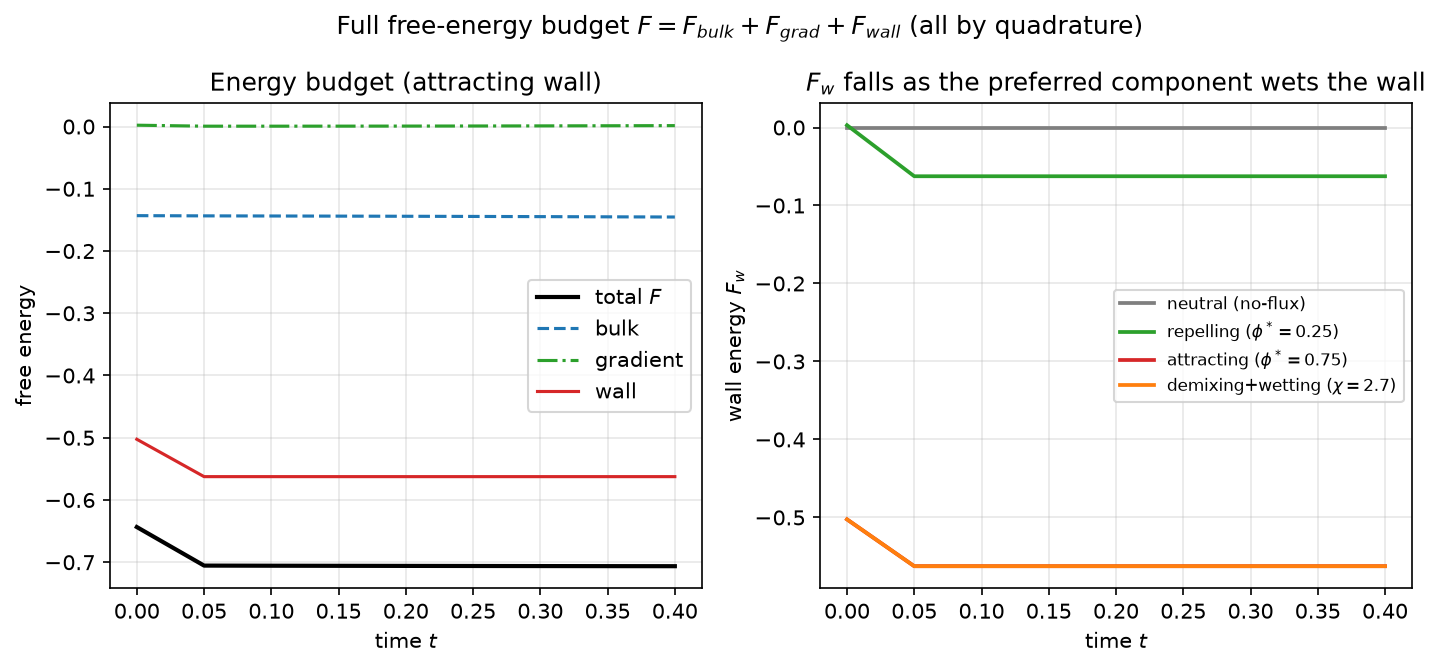
\includegraphics[width=\linewidth]{figures/p3_energy.png}
  \caption{Left: the quadrature energy budget $F=F_{\rm bulk}+F_{\rm
    grad}+F_{\rm wall}$ versus time for the attracting wall. Right: the
    wall energy $F_{\rm wall}(t)$ across cases---it decreases as the
    preferred component enriches the substrate, the surface-energy
    signature of wetting.}
  \label{fig:p3energy}
\end{figure}

\section{Six boundary conditions}

\begin{runbox}
\textbf{Run it.}
\begin{lstlisting}
cd physics/03_ch_substrate_bcs
python run_harness.py --config configs/p3.yaml --mode reference \
    --output outputs/p3 --overwrite
python gen_figures.py --run outputs/p3
\end{lstlisting}
The harness marches six boundary conditions, the boundary-layer
$\delta(\kappa)$ study, and the clipping demonstration, writing
\file{results.json}; \file{gen\_figures.py} renders every figure and the
cited numbers from that saved run. (\file{run.py} is the quick
student self-check for the first three cases.)
\end{runbox}

\begin{figure}[h]\centering
  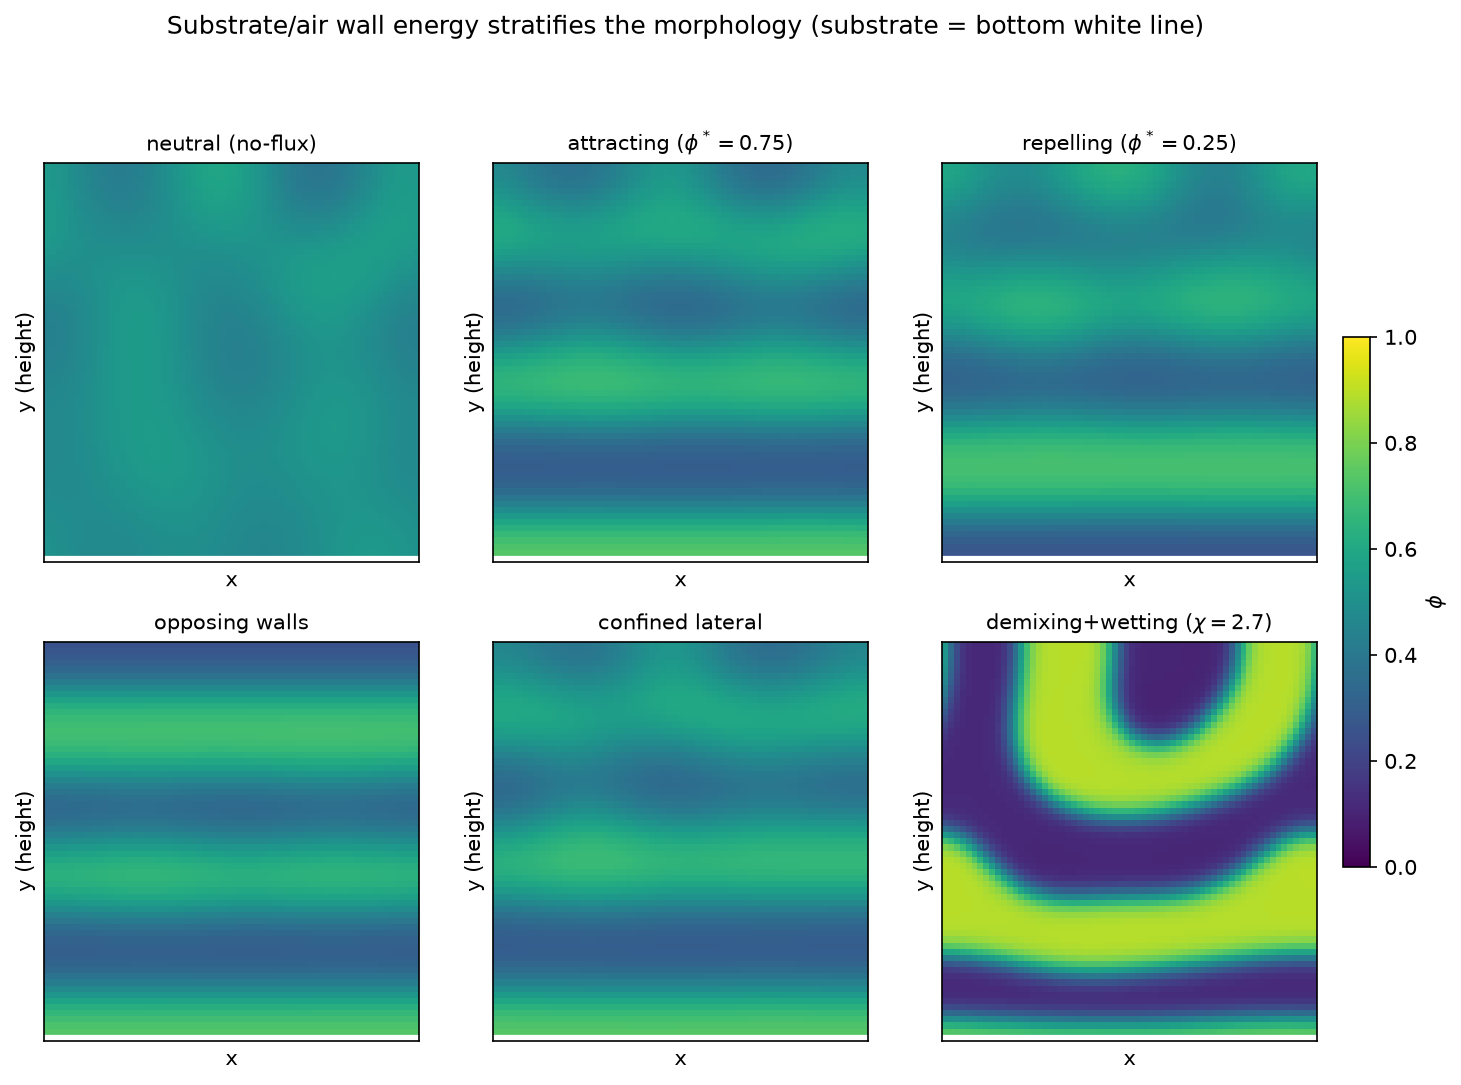
\includegraphics[width=\linewidth]{figures/p3_fields.png}
  \caption{The composition field under the six boundary conditions
    (substrate = the bottom white line). Attracting/demixing walls
    enrich the bottom layer; the repelling wall depletes it; the opposing
    walls enrich the substrate while depleting the air side; the confined
    case replaces the periodic sides with no-flux walls; the neutral wall
    does neither.}
  \label{fig:p3fields}
\end{figure}

\begin{figure}[h]\centering
  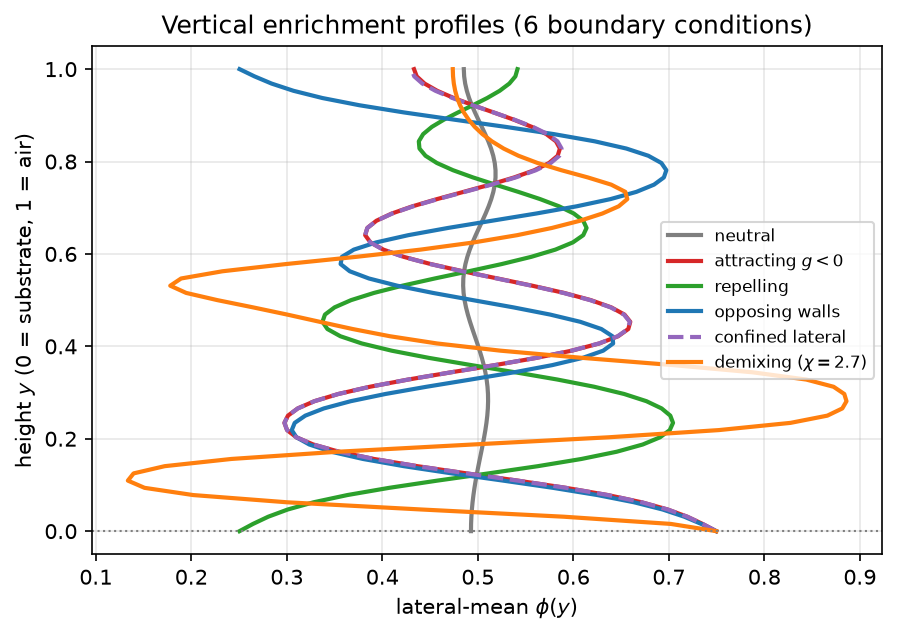
\includegraphics[width=0.66\linewidth]{figures/p3_profiles.png}
  \caption{Vertical enrichment profiles (lateral-mean $\phi$ vs height,
    $0$ = substrate, $1$ = air). The attracting/demixing walls bend the
    profile up at the substrate; the repelling wall bends it down; the
    opposing walls tilt it both ways; the neutral profile is flat. This
    boundary layer is the substrate's fingerprint on the morphology.}
  \label{fig:p3profiles}
\end{figure}

\begin{keybox}
\textbf{Measured self-check} (your harness run should reproduce these).
\begin{center}\small
\begin{tabular}{lcc}
\toprule
case & substrate $\phi$ & enrichment $\Delta\phi$ \\
\midrule
neutral (no-flux)          & \PthreeNeutralSub  & \PthreeNeutralEnr \\
attracting $\phi^\star{=}0.75$ & \PthreeAttractSub  & \PthreeAttractEnr \\
repelling $\phi^\star{=}0.25$  & \PthreeRepelSub    & \PthreeRepelEnr \\
opposing walls             & \PthreeOpposingSub & air $\phi=\PthreeOpposingAir$ \\
confined lateral           & \PthreeConfinedSub & \PthreeConfinedEnr \\
demixing+wetting ($\chi{=}\PthreeChiDemix$) & \PthreeDemixSub & \PthreeDemixEnr \\
\bottomrule
\end{tabular}
\end{center}
Mass drift $\le\PthreeMassdrift$ in \emph{every} case (conservation
survives the wall energy); the substrate composition tracks the preferred
$\phi^\star=-g/(2h)$. The opposing-wall case enriches the substrate
\emph{and} depletes the air face; the confined case (no-flux lateral
sides instead of the periodic film) reaches essentially the same
substrate enrichment---the vertical wall physics is set by the substrate,
not the lateral boundary.
\end{keybox}

\section{The enrichment boundary layer}

The wall preference decays into the film over a length $\delta$. Near the
substrate the excess $\phi(y)-\phi_{\rm bulk}$ relaxes exponentially, and
linearizing \eqref{eq:p3ch} about the bulk gives a decay length
$\delta\sim\sqrt{\kappa/f''}$---so, at fixed $f''$,
$\delta\propto\sqrt{\kappa}$. Measured on a \emph{stable} (sub-spinodal)
bulk---so the only structure in $\phi(y)$ is the wall layer---across four
$\kappa$ values, the $1/e$ decay length fits $\delta\sim\kappa^{\PthreeDeltaSlope}$
($\kappa^{\PthreeDeltaSlopeFit}$ from an exponential fit), both within a
few percent of the predicted $\tfrac12$ (Fig.~\ref{fig:p3bdlayer}): the
layer thickens from $\delta_{1/e}=\PthreeBdDeltaLo$ at
$\kappa=\PthreeBdKappaLo$ to $\PthreeBdDeltaHi$ at $\kappa=\PthreeBdKappaHi$.
This is a \emph{measured} scaling, not an assertion: to make the substrate
layer thinner, lower $\kappa$.

\begin{figure}[h]\centering
  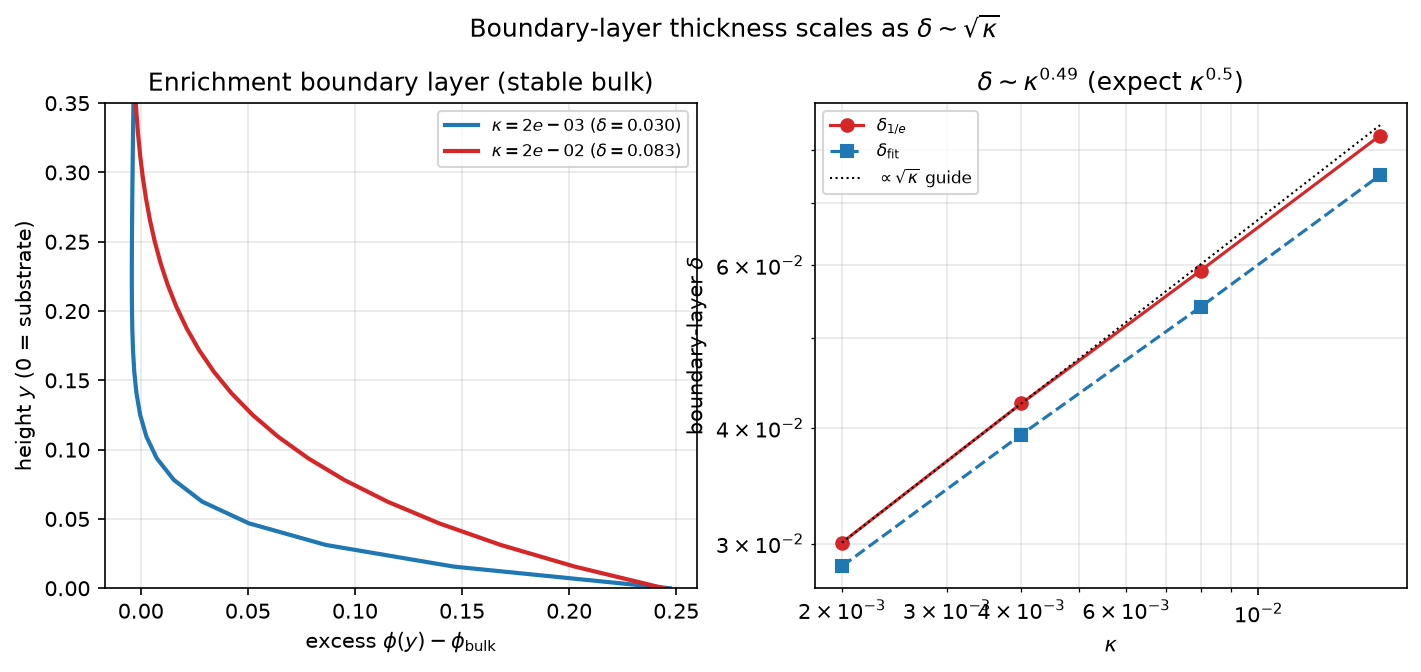
\includegraphics[width=\linewidth]{figures/p3_bdlayer.png}
  \caption{Left: the near-wall excess $\phi(y)-\phi_{\rm bulk}$ and its
    $1/e$ depth. Right: the boundary-layer thickness $\delta$ versus
    $\kappa$ (log--log); both the $1/e$ and exponential-fit lengths track
    the $\sqrt{\kappa}$ guide.}
  \label{fig:p3bdlayer}
\end{figure}

\section{Code walk-through}

\paragraph{1. Turn on the wall.} The substrate energy is three
constructor arguments on the production brick:
\begin{lstlisting}
st = MultiPhaseStepper(dm, M=1, K=0, chi_aa=..., onsager=[[0.2]],
                       wall_g=[-1.5], wall_h=[1.0], wall_face=(1, 0))
\end{lstlisting}
\code{wall\_face=(1,0)} selects the $y=0$ (axis 1, min side) substrate
edge; \code{wall\_g}, \code{wall\_h} are $g,h$ of \eqref{eq:fw}. Setting
both to zero recovers the neutral no-flux boundary bit-for-bit. The
opposing-wall case adds a second face on the air side; the confined case
builds the mesh with no-flux (non-periodic) lateral sides.

\paragraph{2. Where the two boundary integrals live.} In
\file{src/diffsim/physics/multiphase.py} (\code{\_assemble\_host}) the
wall term is the only face integral added---on the $\mu$ rows:
\begin{lstlisting}
# r_mu_i(a) += - INT_w N_a (g_i + 2 h_i phi_i) dS
fw = g_i + 2*h_i * phi_i[wall_faces]
F_full[mu_rows] += einsum("fab,fb->fa", wall_face_M, fw)
# Jacobian: -2 h_i * wall_face_M on the (mu_i, phi_i) block
\end{lstlisting}
The mass-flux condition (a) needs \emph{no} code: leaving the $\phi$ rows
without a face term \emph{is} the natural $\grad\mu\!\cdot\!n=0$.

\paragraph{3. Every number by quadrature.} \file{substrate.py}'s
\code{WallDiagnostics} evaluates $\phi$ and $\grad\phi$ at the Gauss
points and integrates the content, the bulk/gradient energies (volume
quadrature) and the wall energy (surface quadrature on the face mass),
and reports the projection status---all from the shared
\file{diffsim.diagnostics} library, so the document's numbers are the
unit-tested metrics, not a bespoke re-computation.

\section{Explore on your own}

\question{Move $\phi^\star$ toward $0$ or $1$ (increase $|g|$ at fixed
$h$). The bounded well never clips---verify \code{projected\_dofs}$=0$ even
at $\phi^\star=0.99$. Now quench from a violating IC (raise the amplitude)
and watch the projection fire while the converged-state mass stays fixed.
Finally switch to a \emph{linear} wall ($h=0$) and observe the time step
collapse: why is that equilibrium inadmissible? Relate to
Chapter~\ref{ch:p2}.}

\question{Put a wall on the \emph{air} side (\code{wall\_face=(1,1)}) with
the opposite preference---the opposing-wall case. Does the morphology
invert top-to-bottom? What does this imply for which component ends up at
the top vs bottom electrode?}

\question{Raise $\chi$ above the spinodal (the demixing case) so the blend
also phase-separates. Does the attracting wall bias \emph{which} phase
wets the substrate? Compare $F_{\rm wall}$ with the single-phase cases.}

\question{Verify conservation explicitly: track the quadrature mass
$\int\phi\,dV$ over the run for each boundary condition. Why does the wall
energy, unlike a Dirichlet condition, leave the mass exactly fixed---and
why is the nodal-mean a misleading proxy near the wall?}

\question{Measure the boundary-layer thickness at three more $\kappa$
values and confirm $\delta\sim\sqrt{\kappa}$. Why did the scaling study
use a sub-spinodal bulk rather than the demixing $\chi=\PthreeChi$?}

% ====================================================================
